\documentclass[11pt]{beamer}
\usetheme{PaloAlto}
\usepackage[utf8]{inputenc}
\usepackage{amsmath}
\usepackage{amsfonts}
\usepackage{amssymb}

\graphicspath{{pictures/}}
\DeclareGraphicsExtensions{.pdf,.png,.jpg}

\author{Isabella Aspodinger, Alexander Pilan}
\title{Big Data}
\setbeamercovered{transparent} 
\setbeamertemplate{navigation symbols}{} 
%\logo{} 
%\institute{} 
%\date{} 
%\subject{} 
\begin{document}

\begin{frame}
\titlepage
\end{frame}

\begin{frame}{Inhalt}
\tableofcontents
\end{frame}


\begin{frame}{Definition}
\section{Definition}
\begin{itemize}
\item Volume (Datenvolumen)
\item Velocity (Geschwindigkeit der Datenverarbeitung und Veränderungsdynamik)
\item Variety (Vielfalt der Datenstrukturen und -klassen)
\item Veracity (Echtheit der Daten)
\item Value (unternehmerischer Mehrwert)
\item Validity (Datenqualität)
\end{itemize}
\end{frame}


\begin{frame}{Anwendung}
\subsection{Anwendung}
%https://piwikpro.de/blog/was-ist-big-data-und-wie-profitieren-unternehmen-davon/
	\begin{enumerate}
		\item Kundenanalyse
		\item Risikoanalyse
		\item Standortbasiertes Targeting
		\item Kampagneoptimierung
		\item Produktplatzierungsoptimierung
		\item Kriminalistik
		\item Medizin
	\end{enumerate}

\end{frame}


\begin{frame}{Datenherkunft}
\subsection{Datenherkunft}
\begin{enumerate}
\item Aufzeichnungen verschiedenster Überwachungssysteme.
\item die Nutzung von Kunden- oder Bank- bzw. Bezahlkarten 
\item die Nutzung eines Smartphones
\item Social-Media
\item Kraftfahrzeuge
\item vernetzte Technik in Häusern
\item von Behörden und Unternehmen erhobene und gesammelte Daten.

\end{enumerate}

\end{frame}

\begin{frame}{Wachstum von Daten}
\subsection{Wachstum von Daten}
	\begin{figure}
		\center{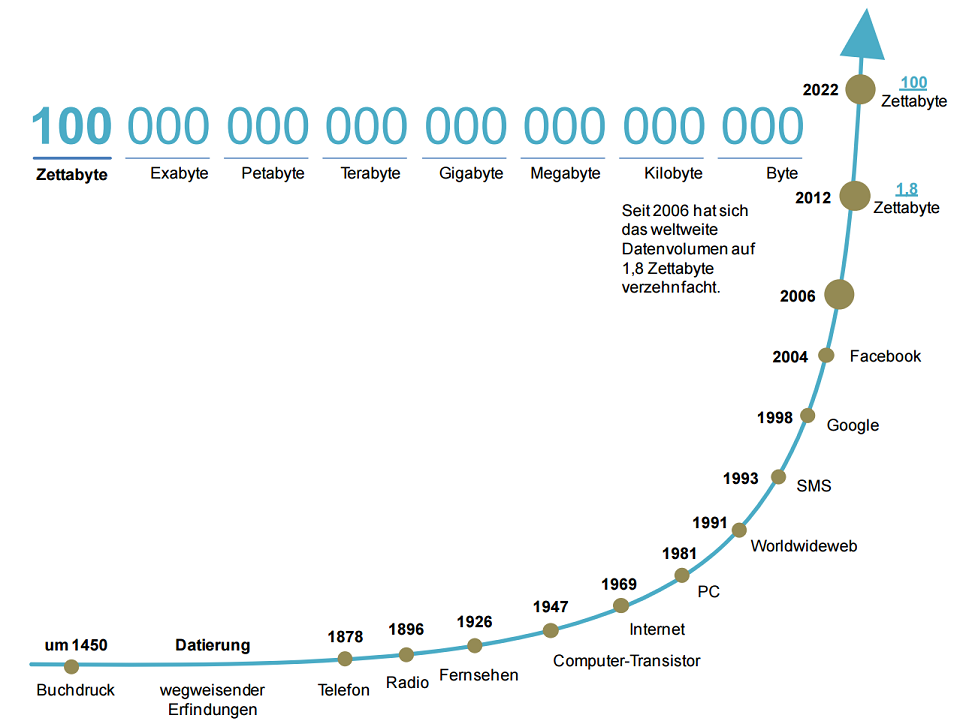
\includegraphics[scale=0.35]{bigdatapng1}}
	\end{figure}
\end{frame}

\begin{frame}{Unterschied}
\subsection{Unterschied}
\begin{table}
\begin{tabular}{|l|l|}

Traditionelle Analytik & Big Data Analytik \\ \hline
Schrittweise Analyse der kleinen Datenmengen & Bearbeitung der ganzen Datenmenge \\ \hline
Abfassung und Sortierung bevor Bearbeitung & Daten werden unverändert bearbeitet \\ \hline
Daten werden angesammelt, bearbeitet, gespeichert und erst dann analysiert & Analyse und Bearbeitung werden je nach Einlauf durchgeführt 
\end{tabular}
\end{table}
\end{frame}


\begin{frame}  {Entwicklungen}
\section{Entwicklungen}
Klassische relationale Datenbanksysteme sowie Statistik- und Visualisierungsprogramme sind oft nicht in der Lage, derart große Datenmengen zu verarbeiten. Für Big Data kommen daher neue Arten von Datenspeicher- und Analyse-Systemen zum Einsatz, die parallel auf bis zu Hunderten oder Tausenden von Prozessoren bzw. Servern arbeiten. Dabei gibt es u. a. folgende Herausforderungen:
\end{frame}
\begin{frame}
\begin{itemize}
\item Verarbeitung vieler Datensätze
\item Verarbeitung vieler Spalten innerhalb eines Datensatzes
\item Schneller Import großer Datenmengen
\item Sofortige Abfrage importierter Daten (Realtime Processing)
\item Kurze Antwortzeiten (Latenz und Verarbeitungsdauer) auch bei komplexen Abfragen
\item Möglichkeit zur Verarbeitung vieler gleichzeitiger Abfragen (Concurrent Queries)
\item Analyse verschiedenartiger Informationstypen (Zahlen, Texte, Bilder, …)

\end{itemize}

\end{frame}

\begin{frame}{NoSQL}
\subsection{NoSQL}
\begin{itemize}
\item Objektdatenbanken
\item Grid- und Cloud-Datenbanken
\item XML-Datenbanken
\item Andere nicht-relationale Datenbanken
\end{itemize}
\end{frame}

\begin{frame}{NoSQL}
\framesubtitle{Kriterien}
\begin{itemize}
\item Nichtrelationales Datenmodell
\item Schemafrei (oder nur schwache Restriktionen)
\item Bieten einfache API
\item Verteilte Architektur, optimiert für einfache Replikation und horizontale \item Skalierung
\item Kein ACID-Konsistenzmodell
\item Open Source
\end{itemize}
\end{frame}

\begin{frame}{NoSQL}
\begin{figure}
		\center{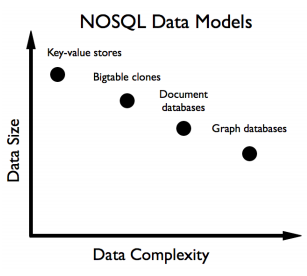
\includegraphics[scale=0.7]{img2}}
\end{figure}
\end{frame}

\begin{frame}{JSON}
\subsection{JSON}
 ist ein kompaktes Datenformat in einer einfach lesbaren Textform zum Zweck des Datenaustauschs zwischen Anwendungen.

\end{frame}

\begin{frame}{Map Reduce}
\subsection{Map Reduce}
\begin{figure}
		\center{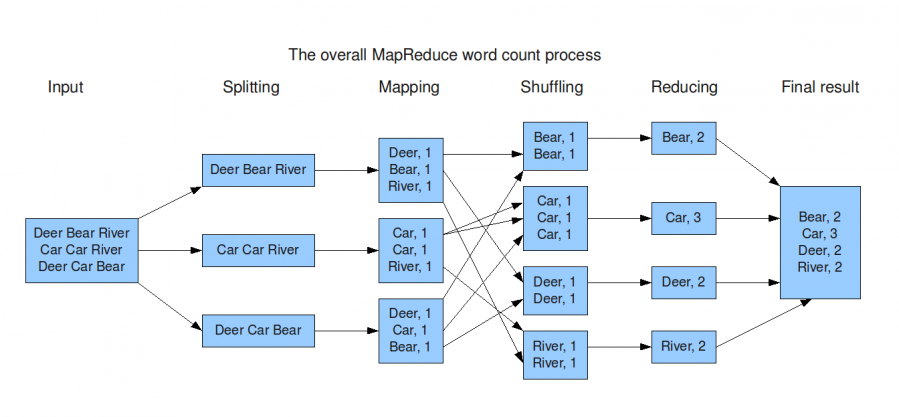
\includegraphics[scale=0.35]{img1}}
\end{figure}
\end{frame}

\begin{frame}{Hadoop}
\subsection{Hadoop}
\begin{center}
\begin{figure}
		\center{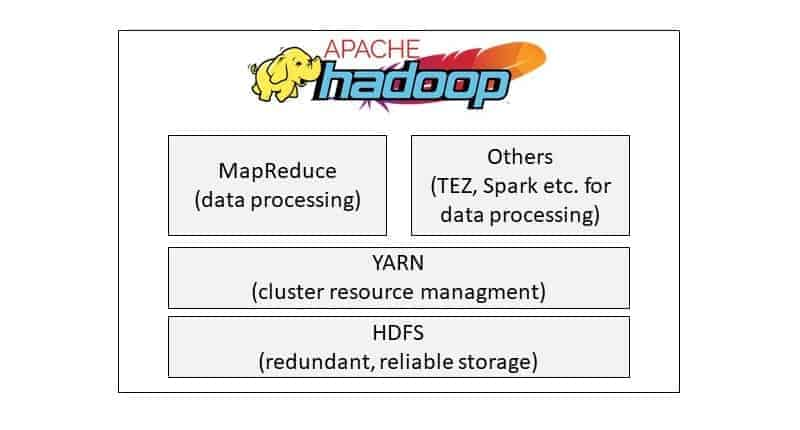
\includegraphics[scale=0.35]{img3}}
\end{figure}
\end{center}
\begin{itemize}
	\item HDFS (Hadoop Distributed File System)
	\item YARN
	\item Map Reduce
\end{itemize}
\end{frame}

\begin{frame}{HDFS}
\begin{center}
\begin{figure}
		\center{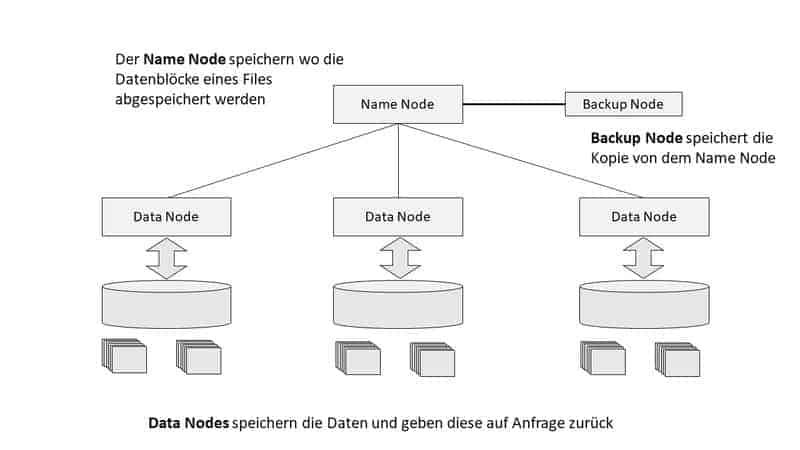
\includegraphics[scale=0.35]{img4}}
\end{figure}
\end{center}
\end{frame}

\begin{frame}{Spark}
\subsection{Spark}


\end{frame}


\end{document}